% Conference talk: 20 minutes + questions.
% Build: make  (pdflatex via latexmk)
\documentclass[aspectratio=169,10pt]{beamer}

\usetheme[progressbar=frametitle,numbering=fraction,sectionpage=none,block=fill]{moloch}
\usefonttheme{professionalfonts}

\usepackage[T1]{fontenc}
\usepackage[sfdefault,book,semibold,lining]{FiraSans}
\usepackage[scaled=0.88]{FiraMono}
\usepackage{newtxsf}

\usepackage{booktabs}
\usepackage{array}
\usepackage{graphicx}
\usepackage{appendixnumberbeamer}
\usepackage{algpseudocode}
\algnotext{EndIf}
\algnotext{EndFunction}
\usepackage{tikz}
\usetikzlibrary{arrows.meta,positioning,calc,shapes.geometric}

\graphicspath{{figures/}}

% ---------------------------------------------------------------- notation
\newcommand{\LeafHash}{\operatorname{LeafHash}}
\newcommand{\NodeHash}{\operatorname{NodeHash}}
\newcommand{\dig}{\operatorname{dig}}
\newcommand{\Tree}{\operatorname{Tree}}
\newcommand{\map}{\operatorname{map}}
\newcommand{\lcp}{\operatorname{lcp}}
\newcommand{\nxt}{\operatorname{next}}
\newcommand{\dom}{\operatorname{dom}}
\newcommand{\cat}{\mathbin{\|}}
\newcommand{\K}{\mathcal{K}}
\newcommand{\V}{\mathcal{V}}
\newcommand{\bits}[1]{\texttt{#1}}

% ---------------------------------------------------------------- colours
% Unicity palette: light grey ground, near-black text, one orange accent.
\definecolor{uBg}{HTML}{F4F5F6}
\definecolor{uInk}{HTML}{141517}
\definecolor{uGrey}{HTML}{585A5E}
\definecolor{uLine}{HTML}{D5D7DA}
\definecolor{uOrange}{HTML}{F25F05}
\definecolor{uPale}{HTML}{FDEBDD}

\molochcolors{
  normal text fg=uInk, normal text bg=uBg,
  alerted text=uOrange, example text=uOrange,
  frametitle fg=uInk, frametitle bg=uBg,
  progressbar fg=uOrange, progressbar bg=uLine,
  title separator=uOrange,
  standout fg=uInk, standout bg=uBg,
}
\setbeamercolor{block title}{fg=uInk, bg=uPale}
\setbeamercolor{block body}{fg=uInk, bg=white}
\setbeamercolor{itemize item}{fg=uOrange}
\setbeamercolor{itemize subitem}{fg=uOrange}
\setbeamercolor{enumerate item}{fg=uOrange}
\setbeamercolor{institute}{fg=uGrey}
\setbeamercolor{footnote mark}{fg=uOrange}

% The theme divides by the total frame count, which is zero for the
% appendix on the first run.
\makeatletter
\setbeamertemplate{progress bar in head/foot}{%
  \nointerlineskip%
  \pgfmathsetlength{\moloch@progressinheadfoot}{%
    \paperwidth * min(1,\insertframenumber/max(1,\inserttotalframenumber))}%
  \begin{beamercolorbox}[wd=\paperwidth]{progress bar in head/foot}
    \begin{tikzpicture}
      \fill[bg] (0,0) rectangle (\paperwidth, \moloch@progressinheadfoot@linewidth);
      \fill[fg] (0,0) rectangle (\moloch@progressinheadfoot, \moloch@progressinheadfoot@linewidth);
    \end{tikzpicture}
  \end{beamercolorbox}%
}
\makeatother

\setbeamertemplate{footnote}{\parindent 0em\noindent\raggedright\tiny\insertfootnotetext\par}

% ---------------------------------------------------------------- diagrams
\definecolor{preserved}{HTML}{E2E4E7}
\definecolor{opened}{HTML}{FFFFFF}
\definecolor{fresh}{HTML}{FBC9A6}
\definecolor{recomp}{HTML}{FDEBDD}
\definecolor{attack}{HTML}{F6C4C5}
\definecolor{attackline}{HTML}{C0282D}

\tikzset{
  box/.style={draw=uGrey, rounded corners=2pt, align=center, inner sep=3pt, font=\footnotesize},
  jn/.style={box, minimum width=1.75cm, minimum height=0.6cm},
  lf/.style={box, minimum width=1.45cm, minimum height=0.6cm},
  arr/.style={-{Latex[length=2mm]}, semithick, uGrey},
  darr/.style={{Latex[length=2mm]}-{Latex[length=2mm]}, semithick, uGrey},
  lbl/.style={font=\scriptsize, inner sep=1.5pt},
  bitlbl/.style={font=\scriptsize, inner sep=1pt},
  ord/.style={font=\scriptsize\bfseries, text=uOrange, inner sep=1pt},
}
\newcommand{\swatch}[1]{\tikz[baseline=-0.6ex]\node[box, fill=#1, minimum width=3mm, minimum height=3mm, inner sep=0]{};}

% ---------------------------------------------------------------- title
\title{Unicity Infrastructure: the Aggregation Layer}
\subtitle{Provably secure add-only dictionaries with succinct consistency proofs}
\author{Risto Laanoja\textsuperscript{1} \and Mike Gault\textsuperscript{1} \and Dirk Draheim\textsuperscript{2} \and Ahto Buldas\textsuperscript{2}}
\institute{\textsuperscript{1}Unicity Labs \qquad \textsuperscript{2}Tallinn University of Technology}
\date{NGISE 2026, Delhi NCR, India, 28--29 October 2026}

\begin{document}

\maketitle

% =====================================================================
\section{Motivation}
% =====================================================================

\begin{frame}{Motivation: the Unicity Network}
\begin{columns}[T]
\begin{column}{0.56\textwidth}
\begin{itemize}
  \item Tokens are self-contained data objects kept by their owners. Transactions are executed and validated off-chain by the parties involved.
  \item There is no global ordering of transactions and no global execution.
  \item The only globally shared state is the set of spent token states, each recorded under the identifier $k = H(\text{token state})$.
  \item A transaction is accepted only together with a \alert{proof of unicity}: an inclusion proof of the spent state against a root certified by the consensus layer.
\end{itemize}
\end{column}
\begin{column}{0.40\textwidth}
\centering
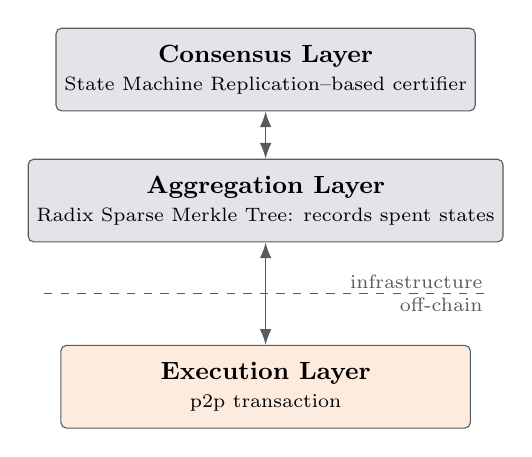
\begin{tikzpicture}[layer/.style={box, minimum width=5.2cm, minimum height=1.05cm, font=\small}]
  \node[layer, fill=preserved] (cl) {\textbf{Consensus Layer}\\[-1pt]\scriptsize State Machine Replication--based certifier};
  \node[layer, fill=preserved, below=6mm of cl] (al) {\textbf{Aggregation Layer}\\[-1pt]\scriptsize Radix Sparse Merkle Tree: records spent states};
  \node[layer, fill=recomp, below=13mm of al] (el) {\textbf{Execution Layer}\\[-1pt]\scriptsize p2p transaction};
  \draw[darr] (cl) -- (al);
  \draw[darr] (al) -- (el);
  \draw[dashed, uGrey] ($(al.south west)!0.5!(el.north west)$) -- ($(al.south east)!0.5!(el.north east)$);
  \node[lbl, anchor=south east, text=uGrey] at ($(al.south east)!0.5!(el.north east)$) {infrastructure};
  \node[lbl, anchor=north east, text=uGrey] at ($(al.south east)!0.5!(el.north east)$) {off-chain};
\end{tikzpicture}
\end{column}
\end{columns}
\end{frame}

% ---------------------------------------------------------------------
\begin{frame}{Motivation: p2p vs online/on-chain transactions}
\begin{itemize}
  \item A recipient can check the validity of a token history offline: signatures, spending predicates, computational integrity proofs.
  \item The statement \emph{``this state has not been spent before''} concerns global view. It cannot be checked based on data object.
  \item A trustless peer-to-peer transaction system therefore needs an online shared record of consumed states, with inclusion and non-inclusion proofs against a unique certified root.\footnote{Assuming no trusted hardware (secure elements, TEEs) and an open set of recipients.}
  \item This record is the \textbf{minimal online component} of an otherwise p2p transaction system. Ordering, execution, and data storage can be left to the transacting parties.
\end{itemize}
\vspace{2mm}
\begin{block}{This work}
A provably secure implementation of this record as an add-only authenticated dictionary. It can be operated by untrusted parties thanks to cryptographic consistency proofs.
\end{block}
\end{frame}



% ---------------------------------------------------------------------
\begin{frame}{Setting: an add-only dictionary}
\small
\begin{itemize}
  \item Key $k = H(\text{state}) \in \K = \{0,1\}^{256}$ identifies a consumed token state. Value $v = H(\text{transaction})$ identifies the transaction that consumed it.
  \item After round $i$ the service commits to a finite partial map $M_i\colon \K \to \V \cup \{\bot\}$ by the digest $r_i$.
  \item Add\footnote{unordered}-only: $M_{i-1} \subseteq M_i$. A key is set once and never changed or removed. Insertion order is not retained, so $r_i$ commits to the map.
\end{itemize}
\vspace{1mm}
\begin{tabular}{@{}llll@{}}
\toprule
Proof & Statement & Verified against & Verified by \\
\midrule
inclusion & $M_i(k) = v$ & $r_i$ & recipients \\
non-inclusion & $M_i(k) = \bot$ & $r_i$ & recipients \\
consistency & $M_{i-1} \subseteq M_i$ & $(r_{i-1}, r_i)$ & consensus layer \\
\bottomrule
\end{tabular}

\vspace{2mm}
\begin{block}{Security}
\footnotesize
(i) From a consistency proof that verifies against $(r_{i-1}, r_i)$, either maps $M_{i-1} \subseteq M_i$ with these digests, or a $H$-collision is extractable.\\
(ii) Proofs of $M(k)=v$ and $M(k)=v'$ with $v \neq v'$ against the same digest yield an $H$-collision.
\end{block}
\end{frame}

% ---------------------------------------------------------------------
\begin{frame}{Setting: Trust model}
\begin{columns}[T]
\begin{column}{0.42\textwidth}
\centering
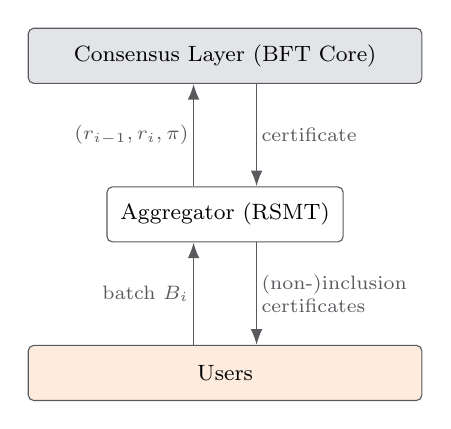
\begin{tikzpicture}
  \node[box, fill=preserved, minimum width=5.0cm, minimum height=0.7cm] (cl) {Consensus Layer (BFT Core)};
  \node[box, fill=white, minimum width=3.0cm, minimum height=0.7cm, below=1.3cm of cl] (ag) {Aggregator (RSMT)};
  \node[box, fill=recomp, minimum width=5.0cm, minimum height=0.7cm, below=1.3cm of ag] (us) {Users};
  \draw[arr] ([xshift=-4mm]ag.north) -- node[lbl, left] {$(r_{i-1}, r_i, \pi)$} ([xshift=-4mm]ag.north |- cl.south);
  \draw[arr] ([xshift=4mm]ag.north |- cl.south) -- node[lbl, right] {certificate} ([xshift=4mm]ag.north);
  \draw[arr] ([xshift=-4mm]us.north -| ag.south) -- node[lbl, left] {batch $B_i$} ([xshift=-4mm]ag.south);
  \draw[arr] ([xshift=4mm]ag.south) -- node[lbl, right, align=left] {(non-)inclusion\\certificates} ([xshift=4mm]us.north -| ag.south);
\end{tikzpicture}
\end{column}
\begin{column}{0.55\textwidth}
\begin{block}{Consensus layer as an oracle}
\footnotesize
\begin{algorithmic}[0]
  \Function{Certify}{$r_i, r_{i-1}, \pi$}
    \If{$r_{i-1} \neq r_{\mathrm{last}} \lor \lnot\,\mathrm{valid}(\pi, r_{i-1}, r_i)$}
      \State \Return $\bot$
    \EndIf
    \State $r_{\mathrm{last}} \gets r_i$;\ \ $i \gets i+1$
    \State \Return $(i, r_i, r_{i-1};\ \sigma_{\mathrm{CL}})$
  \EndFunction
\end{algorithmic}
\end{block}
\small
\begin{itemize}
  \item The certifier is a BFT committee elected by delegated proof of stake. It keeps the latest roots only (not a log).
  \item Each certified root is extended at most once, so the dictionary cannot fork.
  \item The aggregator is untrusted. The proof $\pi$ must establish \alert{consistency}: pre-existing bindings are preserved, and each new leaf is placed at the position determined by its key.
\end{itemize}
\end{column}
\end{columns}
\end{frame}

% =====================================================================
\section{Data structure}
% =====================================================================

\begin{frame}{Data Structures: sparse Merkle tree, radix tree}
\begin{columns}[T]
\begin{column}{0.54\textwidth}
\small
\begin{itemize}
  \item Sparse Merkle tree (SMT): every key is a leaf position in a binary tree of depth 256. Empty subtrees are implicit.
  \item Radix sparse Merkle tree (RSMT): a path-compressed tree that contains only leaves and junctions (bifurcations).
\end{itemize}
\vspace{-2mm}
\begin{align*}
  \LeafHash(k,v) &= H(\texttt{0x00} \cat k \cat v)\\
  \NodeHash(d,p,x,y) &= H(\texttt{0x01} \cat \langle d\rangle \cat \langle p\rangle \cat x \cat y)
\end{align*}
\vspace{-6mm}
\begin{itemize}
  \item $d$ is the bifurcation depth and $p \in \{0,1\}^d$ is the \emph{region}, the prefix shared by all keys below the junction.
  \item Depth and region are absolute, so an insertion does not change the hash of any existing node. Every finite map has exactly one valid RSMT.
\end{itemize}
\end{column}
\begin{column}{0.44\textwidth}
\centering
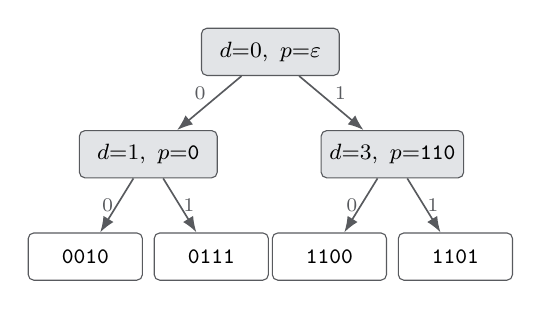
\begin{tikzpicture}[x=1cm,y=1cm]
  \node[jn, fill=preserved] (r) at (0,0) {$d{=}0,\ p{=}\varepsilon$};
  \node[jn, fill=preserved] (l) at (-1.55,-1.3) {$d{=}1,\ p{=}\bits{0}$};
  \node[jn, fill=preserved] (q) at (1.55,-1.3) {$d{=}3,\ p{=}\bits{110}$};
  \node[lf, fill=white] (a) at (-2.35,-2.6) {\bits{0010}};
  \node[lf, fill=white] (b) at (-0.75,-2.6) {\bits{0111}};
  \node[lf, fill=white] (c) at (0.75,-2.6) {\bits{1100}};
  \node[lf, fill=white] (e) at (2.35,-2.6) {\bits{1101}};
  \draw[arr] (r) -- node[bitlbl, above left] {0} (l);
  \draw[arr] (r) -- node[bitlbl, above right] {1} (q);
  \draw[arr] (l) -- node[bitlbl, left] {0} (a);
  \draw[arr] (l) -- node[bitlbl, right] {1} (b);
  \draw[arr] (q) -- node[bitlbl, left] {0} (c);
  \draw[arr] (q) -- node[bitlbl, right] {1} (e);
\end{tikzpicture}

\vspace{2mm}
\raggedright\scriptsize 4-bit keys for illustration. An edge from junction $(d,p)$ on side $\beta$ is valid if the child is deeper than $d$ and its region extends $p \cat \beta$.
\end{column}
\end{columns}
\end{frame}

% ---------------------------------------------------------------------
\begin{frame}{RSMT: justification}
\begin{columns}[T]
\begin{column}{0.54\textwidth}
\small
\begin{itemize}
  \item A certificate holds one sibling digest and one depth per junction on the key path, plus the terminal leaf. For $n$ uniformly distributed keys the expected path length is $\log_2 n + O(1)$, and no binary tree has a mean leaf depth below $\log_2 n$.
  \item Regions are derived from the terminal key and do not make certificate larger.
  \item Inclusion and non-inclusion share one format. If the descent for $k$ ends at a leaf with \emph{another} key, $k$ is absent.
  \item The shape depends only on the key set. There is no rebalancing, and an insertion rehashes only the path to the new leaf.
  \item A batch touches only its frontier, so the consistency proof is linear in the batch size and logarithmic in the tree size.
\end{itemize}
\end{column}
\begin{column}{0.44\textwidth}
\centering
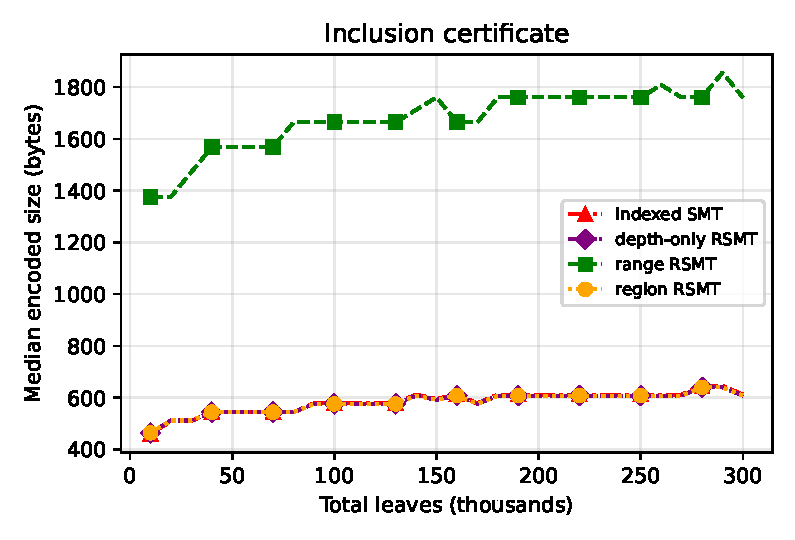
\includegraphics[width=\linewidth]{tree_design_inclusion.pdf}

\raggedright\scriptsize Median certificate size, batches of 10\,000 uniformly distributed keys. In the range variant, every sibling also carries the minimum and maximum key of its subtree.
\end{column}
\end{columns}
\end{frame}

% ---------------------------------------------------------------------
\begin{frame}{Inserting one key}
\centering
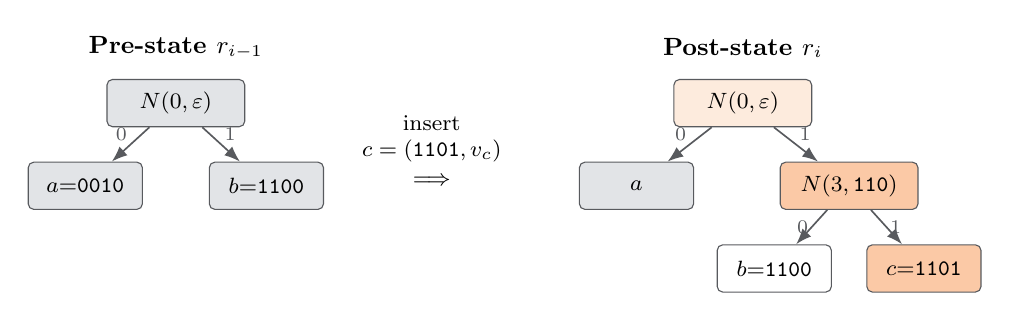
\begin{tikzpicture}[x=1cm,y=1cm]
  % pre-state
  \node[font=\small\bfseries] at (0,0.7) {Pre-state $r_{i-1}$};
  \node[jn, fill=preserved] (o) at (0,0) {$N(0,\varepsilon)$};
  \node[lf, fill=preserved] (oa) at (-1.15,-1.05) {$a{=}\bits{0010}$};
  \node[lf, fill=preserved] (ob) at (1.15,-1.05) {$b{=}\bits{1100}$};
  \draw[arr] (o) -- node[bitlbl, above left] {0} (oa);
  \draw[arr] (o) -- node[bitlbl, above right] {1} (ob);
  % arrow
  \node[align=center, font=\footnotesize] at (3.25,-0.6) {insert\\$c = (\bits{1101}, v_c)$\\[1pt]$\Longrightarrow$};
  % post-state
  \node[font=\small\bfseries] at (7.2,0.7) {Post-state $r_i$};
  \node[jn, fill=recomp] (n) at (7.2,0) {$N(0,\varepsilon)$};
  \node[lf, fill=preserved] (na) at (5.85,-1.05) {$a$};
  \node[jn, fill=fresh] (nj) at (8.55,-1.05) {$N(3,\bits{110})$};
  \node[lf, fill=opened] (nb) at (7.6,-2.1) {$b{=}\bits{1100}$};
  \node[lf, fill=fresh] (nc) at (9.5,-2.1) {$c{=}\bits{1101}$};
  \draw[arr] (n) -- node[bitlbl, above left] {0} (na);
  \draw[arr] (n) -- node[bitlbl, above right] {1} (nj);
  \draw[arr] (nj) -- node[bitlbl, left] {0} (nb);
  \draw[arr] (nj) -- node[bitlbl, right] {1} (nc);
\end{tikzpicture}

\vspace{1mm}
\raggedright\small
\begin{itemize}
  \item Non-inclusion certificate for $k_c$ against $r_{i-1}$: $C = \big((0, h_a);\ (k_b, v_b)\big)$. The descent for $k_c = \bits{1101}$ ends at the leaf $k_b = \bits{1100} \neq k_c$.
  \item Update: $\hat d = |\lcp(k_c, k_b)| = 3$. The derived certificate $C^{+} = \big((3, h_b), (0, h_a);\ (k_c, v_c)\big)$ verifies against exactly one root, $r_i = \NodeHash\big(0, \varepsilon, h_a, \NodeHash(3, \bits{110}, h_b, h_c)\big)$.
  \item The verifier checks $C$ against $r_{i-1}$ and computes $r_i$ itself. The new root is not supplied by the operator, and $C^{+}$ is the inclusion certificate for $c$.
\end{itemize}
\end{frame}

% ---------------------------------------------------------------------
\begin{frame}{Single insertion: proof sketch (of the correctness of the consistency check)}
\small
For a single insertion, the non-inclusion proof doubles as a consistency proof: it determines the new root and transforms into an inclusion proof for the inserted leaf.

\begin{enumerate}
  \item \textbf{Matching.} If an opening tree (a partially opened commitment) evaluates to $\dig(T)$, each opened node equals the node of $T$ at the same position, or a collision of $H$ is computable.
  \item \textbf{Certificate correctness.} The openings of a verifying certificate are the ancestors of its terminal leaf $(k',v')$. The descent is key-directed, so $k' \neq k$ implies $k \notin \dom(M)$.
  \item \textbf{Update theorem.} If $C$ verifies for $k$ against $\dig(\Tree(M))$ and $k' \neq k$, then $\nxt(C;k,v) = \dig\big(\Tree(M \uplus \{k \mapsto v\})\big)$ \footnote{$\uplus$ denotes disjoint union}. The new junction is grafted at depth $|\lcp(k,k')|$.
  \item \textbf{Run soundness.} By induction from $r_0 = \dig(\varnothing)$, every certified run satisfies $r_i = \dig(\Tree(M_i))$, and its keys are pairwise distinct.
\end{enumerate}
\begin{block}{No placement check is needed}
\footnotesize
The post-state is computed from the pre-state, and the regions are derived from the terminal key. The results above also hold for a junction hash that commits to the depth only. A batch of $j$ insertions costs $j$ certificates and $j$ sequential intermediate roots.
\end{block}
\end{frame}

% =====================================================================
\section{Batch consistency}
% =====================================================================

\begin{frame}{Batch insertion: the consistency proof}
\begin{columns}[T]
\begin{column}{0.38\textwidth}
\centering
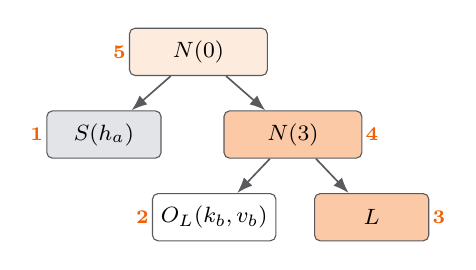
\begin{tikzpicture}[x=1cm,y=1cm]
  \node[jn, fill=recomp, label={[ord]left:5}] (n) at (0,0) {$N(0)$};
  \node[lf, fill=preserved, label={[ord]left:1}] (na) at (-1.2,-1.05) {$S(h_a)$};
  \node[jn, fill=fresh, label={[ord]right:4}] (nj) at (1.2,-1.05) {$N(3)$};
  \node[lf, fill=opened, label={[ord]left:2}] (nb) at (0.2,-2.1) {$O_L(k_b,v_b)$};
  \node[lf, fill=fresh, label={[ord]right:3}] (nc) at (2.2,-2.1) {$L$};
  \draw[arr] (n) -- (na);
  \draw[arr] (n) -- (nj);
  \draw[arr] (nj) -- (nb);
  \draw[arr] (nj) -- (nc);
\end{tikzpicture}

\vspace{1mm}
\scriptsize
\begin{tabular}{@{}l@{\hspace{4mm}}l@{}}
\swatch{preserved} opaque & \swatch{fresh} new \\
\swatch{opened} opened & \swatch{recomp} re-hashed
\end{tabular}
\end{column}
\begin{column}{0.60\textwidth}
\small
\begin{itemize}
  \item The consistency proof $\pi$ is the post-order serialization of the part of the post-state tree that the batch touches, saved as a transcript (details at the next slide).
  \item A verifier stack machine evaluates $\pi$ in one combined pass and computes both pre- and post-state roots. New junctions are skipped on the pre-state and hashed on the post-state computation.
  \item The verifier processes $\pi$ so that it consumes batch elements $L$ in sorted order.
\end{itemize}
\end{column}
\end{columns}

\vspace{2mm}
\footnotesize
\begin{tabular}{@{}lllll@{}}
\toprule
& Opcode & Pre-state digest & Post-state digest & Advice \\
\midrule
1 & $S(h_a)$ & $h_a$ & $h_a$ & $\bot$ \\
2 & $O_L(k_b,v_b)$ & $h_b$ & $h_b$ & $(256, k_b)$ \\
3 & $L$ & $\varnothing$ & $h_c$ & $(256, k_c)$ \\
4 & $N(3)$ & $h_b$ & $h_N = \NodeHash(3,\bits{110},h_b,h_c)$ & $(3,\bits{110})$ \\
5 & $N(0)$ & $\NodeHash(0,\varepsilon,h_a,h_b) = r_{i-1}$ & $\NodeHash(0,\varepsilon,h_a,h_N) = r_i$ & $(0,\varepsilon)$ \\
\bottomrule
\end{tabular}
\end{frame}

% ---------------------------------------------------------------------
\begin{frame}{The transcript language}
\footnotesize
\begin{tabular}{@{}l l l@{}}
\toprule
Opcode & Meaning & Pushes (pre-state, post-state, advice) \\
\midrule
$S(c)$ & untouched subtree, opaque & $(c,\ c,\ \bot)$ \\
$O(d',p',c_l,c_r)$ & untouched junction, opened & $(h,\ h,\ (d',p'))$ with $h = \NodeHash(d',p',c_l,c_r)$ \\
$O_L(k',v')$ & untouched leaf, opened & $(h,\ h,\ (256,k'))$ with $h = \LeafHash(k',v')$ \\
$L$ & new leaf, next batch element $(k,v)$ & $(\varnothing,\ \LeafHash(k,v),\ (256,k))$ \\
$N(d)$ & junction over the two top entries & $(o,\ n,\ (d,p))$, checked as below \\
\bottomrule
\end{tabular}

\vspace{2mm}
\small
At $N(d)$, with children $(o_l, n_l, a_l)$ and $(o_r, n_r, a_r)$:
\begin{enumerate}
  \item \textbf{Edge coherence.} Every advised child $a_x = (\delta, \varrho)$ satisfies $\delta > d$ and $\varrho[d] = \beta_x$, its side bit. The region $p = \varrho[0..d)$ is derived, and all advised children agree on it.
  \item \textbf{Confinement.} If the junction is new ($o_l = \varnothing$ or $o_r = \varnothing$), both children must be advised. An opaque $S$ can only appear under a junction that already existed.
  \item \textbf{Digest match.} $n = \NodeHash(d,p,n_l,n_r)$. The pre-state digest $o$ is $\varnothing$, the digest of the only existing child, or $\NodeHash(d,p,o_l,o_r)$ when both children existed.
\end{enumerate}
Accept iff the batch is consumed and the stack holds a single entry $(r_{i-1}, r_i, \cdot)$.
\end{frame}

% ---------------------------------------------------------------------
\begin{frame}{Adversarial tree builder}
\begin{columns}[T]
\begin{column}{0.57\textwidth}
\small
\begin{itemize}
  \item With single insertions the verifier computes the post-state. In the batch transcript the operator supplies its shape; preserving old hashes does not preserve the dictionary.
  \item Attack on a junction hash that commits to the depth only: let $(k,v)$ be recorded under $r_{i-1}$ with $k[d^*] = 1$. The stream $[S(r_{i-1}),\ L,\ N(d^*)]$ with batch $\{(k,v')\}$ passes all digest checks.
  \item Under $r_i$, $(k,v')$ has a valid inclusion proof and $(k,v)$ does not.
\end{itemize}
\end{column}
\begin{column}{0.41\textwidth}
\centering
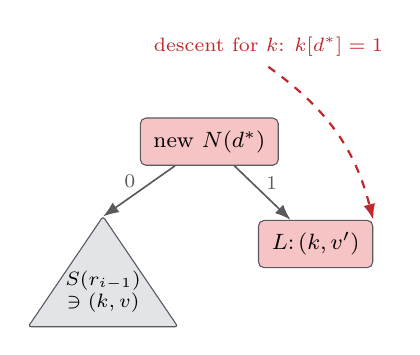
\begin{tikzpicture}[x=1cm,y=1cm]
  \node[jn, fill=attack] (n) at (0,0) {new $N(d^*)$};
  \filldraw[fill=preserved, draw=uGrey, rounded corners=1pt] (-1.35,-0.95) coordinate (apex) -- (-2.3,-2.35) -- (-0.4,-2.35) -- cycle;
  \node[font=\scriptsize, align=center] at (-1.35,-1.9) {$S(r_{i-1})$\\$\ni (k,v)$};
  \node[lf, fill=attack] (l) at (1.35,-1.3) {$L\colon (k,v')$};
  \draw[arr] (n) -- node[bitlbl, above left] {0} (apex);
  \draw[arr] (n) -- node[bitlbl, above right] {1} (l);
  \draw[-{Latex[length=2mm]}, attackline, thick, dashed] (0.75,0.95) node[above, font=\scriptsize] {descent for $k$: $k[d^*]=1$} to[bend left=20] (l.north east);
\end{tikzpicture}
\end{column}
\end{columns}

\vspace{-1mm}
\begin{block}{Fix: region commitment with local opening checks}
\footnotesize
The junction hash commits to the region $p$. Edge coherence is checked wherever an edge is created, and a preserved subtree must be opened where it meets a new junction. In the attack above, the opened old root has a region that is a prefix of $k$, so it cannot be placed on the $0$-side of $N(d^*)$. The region does not make (non)-inclusion certificates larger. As an alternative, committing the key range of every subtree is also sound, but it adds two keys to every certificate sibling.
\end{block}
\end{frame}

% ---------------------------------------------------------------------
\begin{frame}{Batch soundness: proof sketch}
\small
\begin{enumerate}
  \item \textbf{Proof terms.} The verifier accepts $\pi$ iff $\pi$ serializes a unique term $P$ whose attributes satisfy a local predicate at every junction.
  \item \textbf{Old projection.} Removing the $L$ leaves and collapsing new junctions gives an opening tree that evaluates to $r_{i-1}$. Matching places every $S$, $O$, $O_L$ in the pre-state tree $T$.
  \item \textbf{Reconstruction.} Grafting the matched subtrees into $P$ gives $T'$ with $\dig(T') = r_i$. Every edge of $T'$ is an edge of $T$ or passed the coherence check, and confinement excludes an opaque subtree under a new junction.
  \item \textbf{Validity.} $T'$ is a valid tree, so its leaf keys are distinct. The batch keys are fresh, $\map(T') = \map(T) \uplus B$, and $T' = \Tree(M_i)$ by unique representation.
\end{enumerate}
\begin{block}{Theorem (history soundness)}
\footnotesize
Every certified history satisfies $r_i = \dig(\Tree(M_i))$ with $M_i = M_{i-1} \uplus B_i$ for all $i$, or a collision of $H$ is computable from the transcripts.
\end{block}
\footnotesize
Corollaries: one value per key across all roots; no false non-inclusion; no binding outside the batches. The transcript is computed in linear time.
\end{frame}

% =====================================================================
\section{Implementation}
% =====================================================================

\begin{frame}{Scaling: pure transcript}
\centering
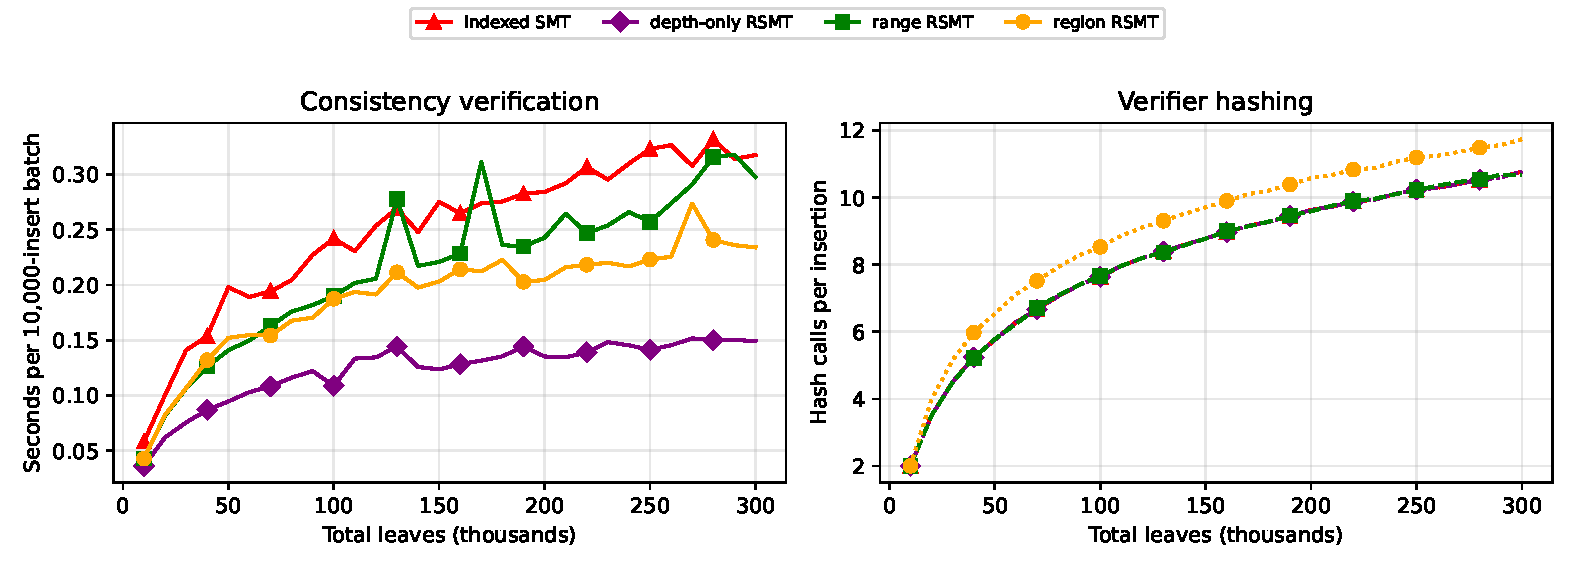
\includegraphics[width=0.8\textwidth]{tree_design_consistency.pdf}

\raggedright\small
\begin{itemize}
  \item Python reference with SHA-256, rounds of 10\,000 uniformly distributed insertions. The depth-only RSMT does not enforce placement and is shown as a lower bound.
  \item Verifier work per insertion grows logarithmically with the tree size.
  \item Transcript and batch take about 320 bytes per insertion at $10^6$ leaves, or 3.2\,MB per round. The consensus layer receives data linear in the transaction rate, which limits this mode to about $10^4$ insertions/s (bandwidth limit).
\end{itemize}
\end{frame}

% ---------------------------------------------------------------------
\begin{frame}{Scaling: STARK-compressed transcript}
\small
The transcript verifier is a custom AIR on Plonky3 (BabyBear field, FRI, no trusted setup). The public input is $(r_{i-1}, r_i)$, and the batch and $\pi$ are witness data.

\vspace{1mm}
\begin{columns}[T]
\begin{column}{0.52\textwidth}
\centering\footnotesize
\begin{tabular}{@{}rrrrr@{}}
\toprule
batch & prove & verify & proof & insertions/s \\
\midrule
1024 & 149\,ms & 44\,ms & 1.69\,MB & 6\,900 \\
4096 & 143\,ms & 45\,ms & 1.76\,MB & 28\,600 \\
8192 & 228\,ms & 47\,ms & 1.82\,MB & 35\,900 \\
\bottomrule
\end{tabular}\\[1mm]
\scriptsize Apple M1 Pro, Poseidon2 as FRI hash.
\end{column}
\begin{column}{0.44\textwidth}
\centering\footnotesize
\begin{tabular}{@{}lrrr@{}}
\toprule
tree hash & cells/call & cells & insertions/s \\
\midrule
Poseidon2 & 300 & $1\times$ & 28\,600 \\
SHA-256 & ${\approx}\,8\,000$ & ${\approx}\,19\times$ & ${\approx}\,1\,500$ \\
\bottomrule
\end{tabular}\\[1mm]
\scriptsize Batch 4096. SHA-256 is analytical result.
\end{column}
\end{columns}

\vspace{1mm}
\begin{itemize}
  \item Verification time does not depend on the batch size. Trace cells are dominated by Poseidon2 permutations (76\,\%).
  %\item SHA-256 estimate, with prove time proportional to trace cells: $0.24 \cdot 1.5 + 0.76 \cdot 0.9 \cdot 8\,000/300 \approx 19$. The other tables widen by 1.5 because digests need 16 limbs instead of 8. A 65-byte leaf or 98-byte node input takes two compressions, against two or three permutations (factor 0.9). A compression commits the bits of $a$, $e$, and $W_t$ in each of 64 rounds, about 8\,000 cells against 300 per permutation.
  \item A general-purpose zkVM (SP1) with a SHA-256 tree hash reached about 1.5 insertions/s.
\end{itemize}
\end{frame}

% ---------------------------------------------------------------------
\begin{frame}{Engineering}
\begin{columns}[T]
\begin{column}{0.40\textwidth}
\centering
\vspace{3mm}
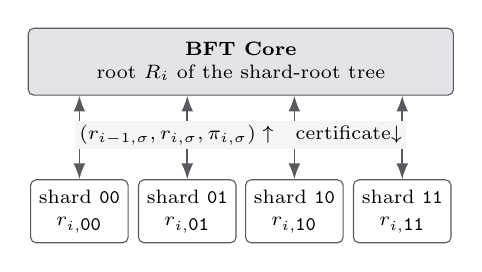
\begin{tikzpicture}[sh/.style={box, minimum width=1.15cm, minimum height=0.8cm, font=\scriptsize}]
  \node[box, fill=preserved, minimum width=5.4cm, minimum height=0.85cm, font=\scriptsize] (core) at (0,1.9) {\textbf{BFT Core}\\root $R_i$ of the shard-root tree};
  \foreach \s/\x in {00/-2.05,01/-0.68,10/0.68,11/2.05} {
    \node[sh, fill=white] (s\s) at (\x,0) {shard $\bits{\s}$\\$r_{i,\bits{\s}}$};
    \draw[darr] (s\s.north) -- (s\s.north |- core.south);
  }
  \node[lbl, fill=uBg, align=center] at (0,0.97) {$(r_{i-1,\sigma}, r_{i,\sigma}, \pi_{i,\sigma})\uparrow$\quad certificate$\downarrow$};
\end{tikzpicture}
\end{column}
\begin{column}{0.6\textwidth}
\small
\begin{itemize}
  \item \textbf{Sharding.} The key prefix $\sigma$ selects the shard. A certificate is the shard's hash path plus $|\sigma|$ digests of the small shard-root tree.
  \item A shard splits further into $\sigma\cat\bits{0}$ and $\sigma\cat\bits{1}$ trivially: each child root is an existing subtree (or $\bot$).
  \item \textbf{Succinct proofs.} Consensus Layer verifies one proof per changed shard. Its load grows with the number of shards, not with the transaction rate.
  \item \textbf{Scaling beyond RAM.} The Rust aggregator keeps the RSMT in on-disk k-v store and loads nodes on demand. The next round runs speculatively while the current root awaits certification.
  \item \textbf{Consistency of full history.} SP1 (zkVM) folds all shard proofs and root transitions into one constant-size STARK proof. Validating it replaces trust in the economical security of the Consensus Layer.
\end{itemize}
\end{column}
\end{columns}
\end{frame}

% =====================================================================
\section{Discussion}
% =====================================================================

\begin{frame}{The Unicity Network: resulting properties}
\begin{columns}[T]
\begin{column}{0.48\textwidth}
\begin{block}{The infrastructure}
\small
\begin{itemize}
  \item records two 32-byte digests per spent token state,
  \item certifies one root per shard and round,
  \item serves inclusion and non-inclusion proofs,
  \item proves its own state transitions.
\end{itemize}
\end{block}
\end{column}
\begin{column}{0.48\textwidth}
\begin{block}{The infrastructure does not}
\small
\begin{itemize}
  \item order or execute transactions,
  \item store token data or transaction payloads,
  \item publish anything except unlinkable state and transaction identifiers.
\end{itemize}
\end{block}
\end{column}
\end{columns}

\vspace{4mm}
\begin{columns}[T]
\begin{column}{0.31\textwidth}\centering
{\Large\bfseries\color{uOrange} $>$10\,000}\\[1pt]\footnotesize insertions per shard, proved locally
\end{column}
\begin{column}{0.31\textwidth}\centering
{\Large\bfseries\color{uOrange} $<$50\,ms}\\[1pt]\footnotesize to verify consistency of a round, independent of the batch size
\end{column}
\begin{column}{0.31\textwidth}\centering
{\Large\bfseries\color{uOrange} 1 proof}\\[1pt]\footnotesize of constant size for the full history since genesis
\end{column}
\end{columns}

\vspace{4mm}
\small To our knowledge, this is the first blockchain design in which the complete server-side state transition history is proven succinctly on commodity hardware.
\end{frame}


% ---------------------------------------------------------------------
\begin{frame}{Summary}
\begin{itemize}
  \item A uniqueness service is the minimal online component of a trustless transaction system. Computational integrity proofs do not replace it.
  \item We implement it as an add-only dictionary on a region-committing radix Merkle tree, with compact inclusion and non-inclusion certificates.
  \item Single insertion consistency is proven by non-inclusion certificates. The batch insertion proof in the transcript forn adds checked coherent placement. In both cases, append-only consistency of the whole certified history reduces to collision resistance of the hash function.
  \item A custom AIR proves more than 10\,000 insertions/s per shard on one CPU. Recursive aggregation gives one constant-size proof of the full history.
\end{itemize}
\end{frame}

% ---------------------------------------------------------------------
\begin{frame}{More information}
\begin{itemize}
  \item Technical report (full proofs, AIR design, aggregation):\\
        \url{https://arxiv.org/pdf/2608.05316}
  \item Aggregator implementation (Rust, disk-backed RSMT, consistency proofs):\\
        \url{https://github.com/ristik/rugregator}
  \item AIR implementation (Plonky3):\\
        \url{https://github.com/ristik/rsmt-air}
    \item Scaling experiments (Python):\\
        \url{https://github.com/ristik/ndsmt-experiments}
  \item Unicity Network:\\
        \url{https://unicity.network}\quad \url{https://github.com/unicitynetwork}
\end{itemize}
\vspace{6mm}
\centering\large Questions
\end{frame}

% =====================================================================
\appendix
\section*{Backup}
% =====================================================================

\begin{frame}
\insertsectionhead
\end{frame}

% ---------------------------------------------------------------------
\begin{frame}{Why the service is ``trustless''}
\footnotesize
\begin{tabular}{@{}>{\raggedright}p{1.9cm} >{\raggedright}p{3.3cm} >{\raggedright}p{3.2cm} >{\raggedright\arraybackslash}p{4.3cm}@{}}
\toprule
Party & Can affect & Cannot affect & Mechanism \\
\midrule
Aggregator & liveness (censorship of requests) & append-only consistency, uniqueness of bindings & consistency proof verified before certification \\
\addlinespace
BFT quorum & liveness; uniqueness of the latest root, by signing two continuations & correctness of the recorded history & aggregate STARK over all rounds; conflicting signed roots are evidence of equivocation \\
\addlinespace
Other users & their own tokens & tokens of others & recipients verify certificates offline \\
\bottomrule
\end{tabular}

\vspace{3mm}
\small
\begin{itemize}
  \item \textbf{Fast path (seconds).} A certificate is validated against the Unicity Trust Base, the record of validator sets. This path assumes an economically motivated BFT quorum.
  \item \textbf{Audit path (minutes to hours).} One recursive STARK covers every round since genesis and makes no assumption about the validators.
  \item Assumptions are collision resistance of $H$ and soundness of the STARKs. No proof system can exclude equivocation; it is detectable and attributable though.
\end{itemize}
\end{frame}

% ---------------------------------------------------------------------
\begin{frame}{Comparison}
\footnotesize
\begin{tabular}{@{}>{\raggedright}p{2.5cm} >{\raggedright}p{2.9cm} >{\raggedright}p{3.4cm} >{\raggedright\arraybackslash}p{3.8cm}@{}}
\toprule
& Shared structure & Statement proved & Prover and granularity \\
\midrule
Merkle logs, Certificate Transparency & chronological append-only log & new log extends the old one (hash-based) & log operator, per pair of tree heads \\
\addlinespace
Nullifier-based chains (Zcash, Aztec) & nullifier set and note commitment tree & spender knows an unspent note (ZK) & user per transaction; in rollups also the operator, with execution \\
\addlinespace
Validity rollups (zkEVM) & VM state trie & correct execution of all transactions & operator or proving market, per block, GPU clusters \\
\addlinespace
\textcolor{uOrange}{This work} & keyed add-only dictionary (RSMT) & append-only consistency of a dictionary update & aggregator on one CPU, per shard and round \\
\bottomrule
\end{tabular}

\vspace{3mm}
\small
\begin{itemize}
  \item A Merkle log has no key-determined positions. In a keyed dictionary a double-spend is a key collision, which the consistency proof excludes.
  \item The circuit contains no transaction execution, signatures, or privacy constraints. Its size depends on the batch size and logarithmically on the tree size.
\end{itemize}
\end{frame}


\begin{frame}{What uniqueness and computational integrity enable}
\footnotesize
A single-assignment register per key is a universal primitive. A shared object can be implemented as a chain of registers keyed by (object identifier, sequence number), cf.\ sticky bits (Plotkin 1989). Any state machine with provable transitions can therefore be advanced with a uniqueness guarantee, and expressiveness is not the limit.

\begin{block}{Limits}
\footnotesize
\begin{enumerate}
  \item \textbf{Contention.} Each transition of an object needs a certified root before the next one can be validated, so one object advances by about one transition per round. A heavily shared object (an order book, an AMM pool) needs an operator that batches requests, which is a rollup on top of the service.
  \item \textbf{Data availability.} The service stores commitments only, and the holder of a state must keep its data. For single-owner assets the owner has this incentive; for shared objects availability must be arranged separately.
  \item \textbf{Online spending.} The recipient needs a fresh inclusion proof. Preventing double-spending offline requires trusted hardware.
  \item \textbf{External facts.} A proof covers a computation on given inputs. Prices, identities, and wall-clock time need oracles.
  \item \textbf{Certifier equivocation.} No proof system can exclude a quorum that signs two continuations. It can be detected and attributed.
\end{enumerate}
\end{block}
\end{frame}

% ---------------------------------------------------------------------
\begin{frame}{Scope of the in-circuit statement}
\small
The consistency proof enforces append-only consistency: prior-state preservation, $\forall k \in \dom(M_{i-1})\colon M_i(k) = M_{i-1}(k)$, and coherent placement of every inserted leaf. The other properties of the service are handled outside the circuit.

\vspace{2mm}
\footnotesize
\begin{tabular}{@{}>{\raggedright}p{3.0cm} >{\raggedright}p{4.4cm} >{\raggedright\arraybackslash}p{5.6cm}@{}}
\toprule
Property & Effect of a violation & Handling \\
\midrule
Request liveness & some users are not served & replicated aggregators; resubmission through another aggregator of the shard \\
Request accountability & an accepted request is omitted & the recipient requests an inclusion certificate against the certified root \\
No phantom inserts & the operator records extra keys & harmless: the keys are fresh and cannot affect existing tokens \\
Unique tree shape & none: implied & follows from the local validity conditions by induction from the empty tree \\
\textcolor{uOrange}{Append-only consistency} & history rewrite, double-spending & \textcolor{uOrange}{proved in the circuit before certification} \\
\bottomrule
\end{tabular}

\vspace{2mm}
\small The circuit asserts the existence of canonical inserted leaves. The batch contents are not public inputs.
\end{frame}

% ---------------------------------------------------------------------
\begin{frame}{AIR layout}
\small
Seven AIR tables share one batch-STARK commitment and are connected by LogUp relations.

\vspace{1mm}
\footnotesize
\begin{tabular}{@{}l >{\raggedright\arraybackslash}p{12.4cm}@{}}
\toprule
A & one row per opcode: pre- and post-state digests, advice $(\delta,\varrho)$, start of the post-order subtree; the last row is bound to $(r_{i-1}, r_i)$ \\
B & every Poseidon2 permutation (width 16), eight lanes per row; occurrences are counted, not deduplicated \\
L & new and opened leaves: 26 range-checked radix-$2^{10}$ digits each for key and value, three sponge steps \\
J & junctions: contiguous post-order children, derived region, depth increase, side bit, confinement, pre-state rule \\
O & openings: canonical left-aligned $d$-bit region, node hash \\
R, P & fixed range table $\{(b,x) : 0 \le b \le 10,\ x < 2^b\}$ and powers of two \\
\bottomrule
\end{tabular}

\vspace{2mm}
\small
\begin{itemize}
  \item The verifier's stack is not materialized. Each non-root row is consumed exactly once as a child of a later junction row, with digest and advice in one lookup tuple.
  \item The subtree-start recurrence makes child indices strictly decrease, which excludes cycles without a cryptographic assumption.
  \item Topology and coherence force the keys of $L$ rows into strictly increasing order, so no separate batch table is needed.
\end{itemize}
\end{frame}

% ---------------------------------------------------------------------
\begin{frame}{Choice of FRI hash}
\begin{columns}[T]
\begin{column}{0.45\textwidth}
\centering\small
\begin{tabular}{@{}lrrr@{}}
\toprule
FRI hash & prove & verify & proof \\
\midrule
Poseidon2 & 138\,ms & 41\,ms & 1.76\,MB \\
SHA-256 & 149\,ms & 18\,ms & 1.69\,MB \\
Blake3 & 130\,ms & 12\,ms & 1.69\,MB \\
\bottomrule
\end{tabular}\\[1mm]
\scriptsize Batch 4096. The tree hash is Poseidon2 in all rows.
\end{column}
\begin{column}{0.52\textwidth}
\small
\begin{itemize}
  \item The FRI and trace-commitment hash is independent of the tree hash and has little effect on prove time.
  \item A native verifier such as BFT Core is about three times faster with Blake3.
  \item Shard proofs for recursive aggregation use the SHA-256 configuration, because FRI Merkle-path hashing maps onto the SHA-256 precompile of the SP1 zkVM.
\end{itemize}
\end{column}
\end{columns}
\end{frame}


% ---------------------------------------------------------------------
% \begin{frame}<presentation:0>
\begin{frame}{Computational integrity does not provide uniqueness}
\begin{columns}[c]
\begin{column}{0.56\textwidth}
\small
\begin{itemize}
  \item A succinct proof $\pi$ attests that the state $s$ results from a valid computation, for example from genesis.
  \item The pair $(s,\pi)$ is data. It can be copied together with its execution environment, and both copies can be continued. The transitions $s \to s'$ and $s \to s''$ are then both provably valid, which is a double-spend or a fork.
  \item The missing primitive is a certificate that $s$ was consumed at most once, that is, a single assignment to the key $H(s)$.
  \item Combined, $\pi$ proves that a transition is valid, and an inclusion proof of $H(s) \mapsto H(t)$ against a certified root proves that it is the only one.
\end{itemize}
\end{column}
\begin{column}{0.42\textwidth}
\centering
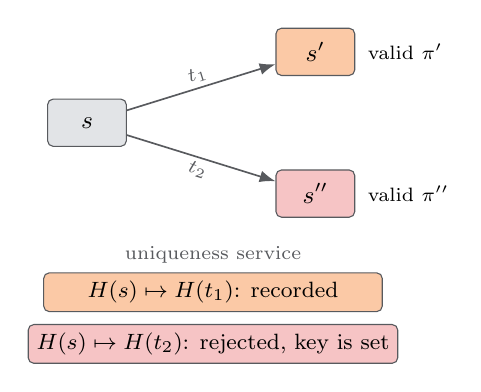
\begin{tikzpicture}[st/.style={box, minimum width=1.0cm, minimum height=0.6cm, font=\small}]
  \node[st, fill=preserved] (s) at (0,0) {$s$};
  \node[st, fill=fresh] (s1) at (2.9,0.9) {$s'$};
  \node[st, fill=attack] (s2) at (2.9,-0.9) {$s''$};
  \draw[arr] (s) -- node[lbl, above, sloped] {$t_1$} (s1);
  \draw[arr] (s) -- node[lbl, below, sloped] {$t_2$} (s2);
  \node[lbl, right=1mm of s1, align=left] {valid $\pi'$};
  \node[lbl, right=1mm of s2, align=left] {valid $\pi''$};
  \node[box, fill=fresh, anchor=north, minimum width=4.3cm] (r1) at (1.6,-1.9) {$H(s) \mapsto H(t_1)$: recorded};
  \node[box, fill=attack, below=1.5mm of r1, minimum width=4.3cm] (r2) {$H(s) \mapsto H(t_2)$: rejected, key is set};
  \node[lbl, above=0.5mm of r1, text=uGrey] {uniqueness service};
\end{tikzpicture}
\end{column}
\end{columns}
\end{frame}
% ---------------------------------------------------------------------
\begin{frame}{Full-history aggregation}
\small
\begin{itemize}
  \item Public values $\mathrm{pv}_n = (\alpha, g, n, c_n, R_n, D_n)$: network identifier, genesis digest, round, sharding-scheme commitment, global root, and a Merkle Mountain Range $D_n$ over $(j, c_j, R_j)_{j \le n}$.
  \item Statement: starting from $g$, in every round $i \le n$ each changed shard root has a verifying consistency proof, every shard split is authenticated, $R_i$ is the root of the current shard roots, and $D_i$ extends $D_{i-1}$ by $(i, c_i, R_i)$.
  \item Step $i$ in the SP1 zkVM verifies the proof of step $i-1$ and the shard STARKs of the rounds it folds. Validator signatures are not part of the statement, and anyone can run the prover on the public round artifacts.
\end{itemize}
\begin{block}{Audit by a user}
\footnotesize
Verify $\Pi_n$ against the verifying-key digest and $(\alpha, g)$. For each certificate of round $j \le n$ in a token's history, check that $(j, c_j, R_j)$ is in $D_n$. Validate younger certificates against the Trust Base and re-audit at the next checkpoint.
\end{block}
\end{frame}

\end{document}
